\chapter{实验}
\label{chap:experiment}
在实验部分,我们通过让游戏AI对战固定场次来判断其强度。也就是说,若某个玩家的胜率越高,则其强度越强。由于缺乏职业玩家与普通玩家的大量数据,我们无法使用Elo rating对AI玩家的强度进行打分\cite{glickman1999rating}。
在目前的硬件条件下,我们支持图\ref{fig:sstate}中所示4种开局,白色方总是先攻,对战双方每50局互换先手,每100局更换开局棋盘,一共对战400局。
\begin{figure}[H]
    \centering
    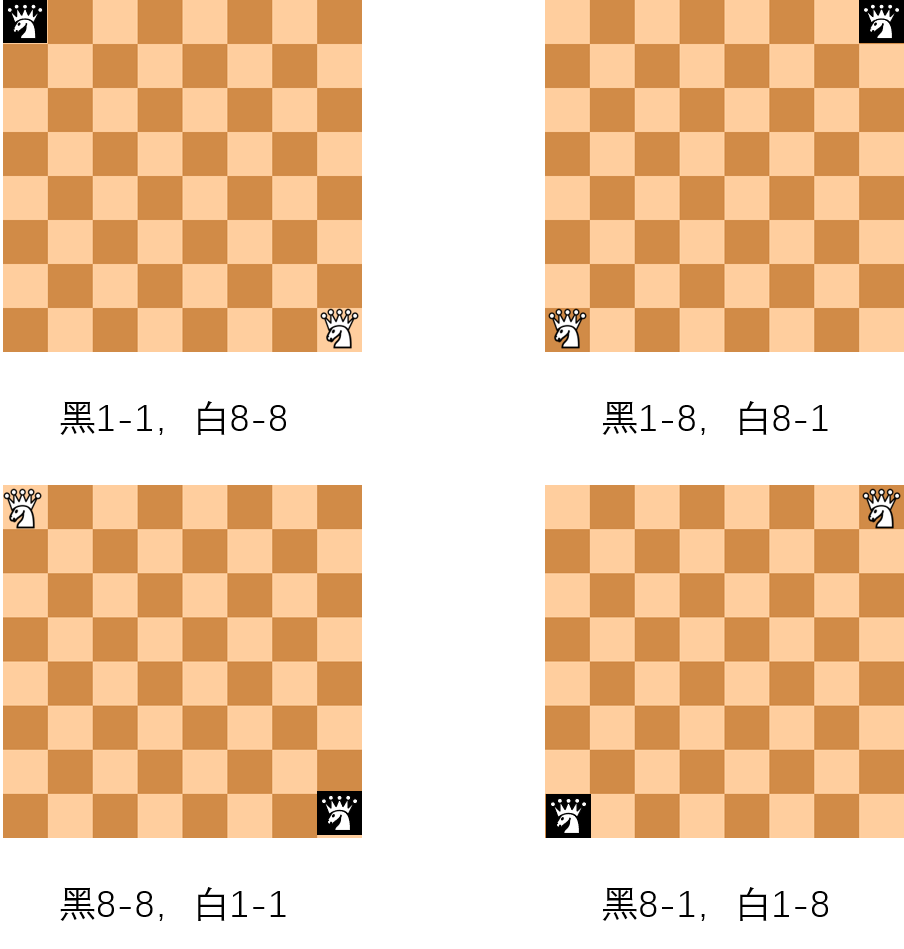
\includegraphics[width=0.8\textwidth]{sstate.PNG}
    \caption[sstate]{%
        超级皇后对战的4种开局%
      }
    \label{fig:sstate}
\end{figure}
对于随机玩家,贪婪玩家与Alpha-beta剪枝玩家这三个基准玩家而言,在任意规则下,其强度排序为Alpha-beta剪枝玩家$>$贪婪玩家$>$随机玩家。具体对局数据如图\ref{fig:baseresult}所示,先手与后手的对战结果合并计算,包含骑士、皇后与超级皇后三种规则状态,随机玩家简写作RP,贪婪玩家简写作GP,Alpha-beta剪枝玩家简写作ABP。
\begin{figure}[H]
    \centering
    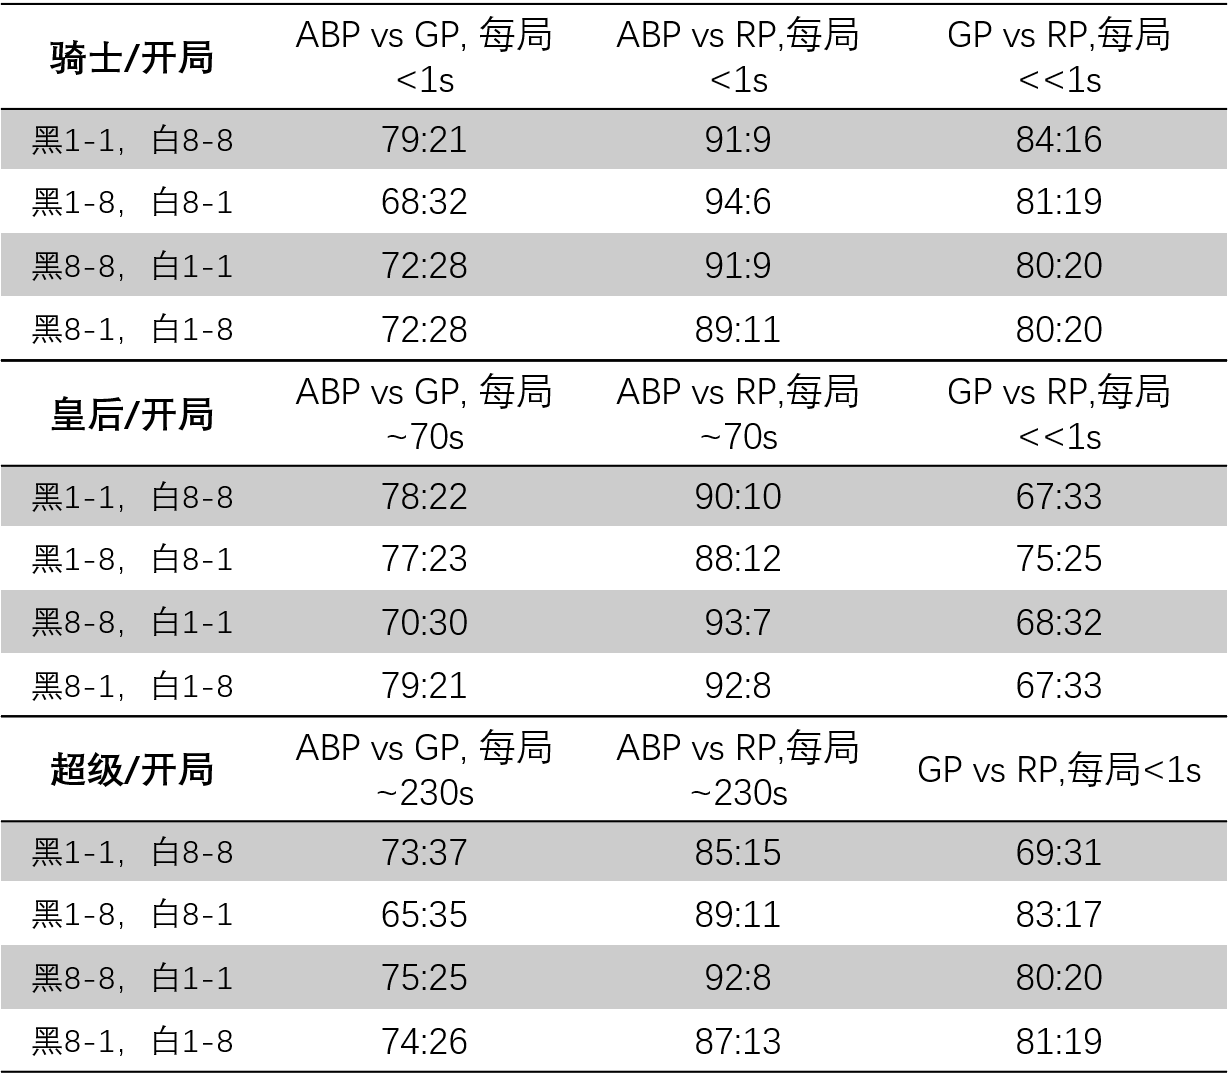
\includegraphics[width=0.8\textwidth]{baseplayer.PNG}
    \caption[baseresult]{%
        基准玩家测试%
      }
    \label{fig:baseresult}
\end{figure}
\section{强化学习训练}

\section{强度测试}

\subsection{随机玩家}

\subsection{贪婪算法玩家}

\subsection{Alpha-beta剪枝玩家}

\subsection{人机对战}
在人机对战环节

